\documentclass[a4paper]{scrartcl} 
\usepackage[T1]{fontenc} 
\usepackage[utf8]{inputenc} 
\usepackage[english]{babel}
\usepackage{color}
\usepackage{graphicx}
\usepackage{subfigure}
\usepackage[scaled=.90]{helvet}
\usepackage{courier}
\usepackage{float}
\usepackage[a4paper, left= 2cm, textwidth=17cm]{geometry}
\usepackage[hidelinks]{hyperref}

\makeatletter         
\def\@maketitle{
\raggedleft

\includegraphics[width = 50mm]{TULOGO.png}\\[8ex]
\begin{center}
{\Huge \bfseries \sffamily \@title }\\[4ex] 
{\Large  \@author}\\[4ex] 
\@date\\[8ex]
\end{center}}
\makeatother

\pagenumbering{gobble}
\begin{document} 

\begin{titlepage}
	\centering
	
\includegraphics[width=0.35\textwidth]{TULOGO.png}\par\vspace{1cm}
	{\scshape\Large \par}
	\vspace{1.5cm}
	{\LARGE\bfseries Course-Project: Finding Dynamic Dead Writes\par}
	{\large\bfseries Program Testing and Analysis WS 2017/2018\par}
	\vspace{2cm}
	\begin{center}
	
\includegraphics[width = 130mm]{Titlepage.jpg}
	\end{center}
	{\Large\itshape Kai-Nico Nase (2644914) and Nicolas Voigt (1289808)\par}
	
	\vfill
	supervised by\par
	Dr. Michael \textsc{Pradel}\\
	and\\
	Jibesh \textsc{Patra}	
    
	\vfill
	{\large \today\par}
\end{titlepage}

\newpage
\tableofcontents
\listoffigures% Abbildungsverzeichnis
\newpage

\pagenumbering{arabic}
\section{Abstract}
This report reflects the progress and results of a Course-Project called "Finding Dynamic Dead Writes" that is part of the subject "Program-Testing and Analysis" at TU-Darmstadt. The first part lists tasks of the task-sheet up that are to be performed. The section "Introduction" describes in general which first steps have been taken to solve the tasks together in teamwork and which tools have been used, to simplify many things. The following sections describe then the definition of a "Dead-Write", which initial tests were carried out and of which components our project consists of. Then the approach and the implementation or components of our code analysis, which is able to detect certain types of "Dead-Writes" and afterwards cleanly remove them will be presented. 
Then some sample programs are listed up that contain different types of dead-writes, which our written Jalangi-Code-Analysis should be able to cleanly remove. At the end, special problems that occurred during our work on the project will be explained, as well as the final results and an outlook.
\section{Goals from the Tasks-Sheet}
\begin{enumerate}
\item The goal of this project is to write a Jalangi [1] analysis that will find dead writes during the execution of JavaScript programs. The analysis should guarantee that some writes are dead for some possible
executions of the program. Given a JavaScript program, the output of the project will be the program without the dead writes
\item Write few simple JavaScript programs that contain dead writes 
\item Get familiar with Jalangi2 and design and implement a Jalangi based analysis that finds dynamic dead writes
\item Validate your implementation with the self-written programs
\item Parse each program using esprima to generate an AST. Traverse the AST using estraverse and
delete the identify dead writes
\item For the final evaluation, use the JavaScript libraries Backbone, Backbone LayoutManager,BigNumber, Bootstrap Datepicker, Cal-Heatmap, Countdown,
Underscore. These libraries have available tests. Run your analysis while executing these tests
\item Remove the dead writes and run the tests again to see if any of them fail.
\item Report your results using the following questions:
\begin{itemize}
      \item{Overall, what percentage of writes are dead?}
      \item{What is the difference in size (bytes) of the program after removing the dead writes.}
      \item{Is there any noticeable performance improvements after removing the dead writes?}
    \end{itemize}
Bonus points: Apart from the given packages, identify 5 node packages that have available
tests and run your analysis on them.
\end{enumerate}
\newpage
 \section{Introduction}
At the begin and after the first briefly meeting with our course-mentor, we discussed "live" first, how to configure our Test-Environment and how would be the best way to share the work, respectively "Who takes which part". Via GitHub, we set up a repository in order to keep our project-files always up to date. Due to the fact that we both live farther away from each other, we decided to hold our regular team meetings online via a free version of the Teamviewer[3] software. We also agreed at the beginning that we would like to create(for this report) diagrams or graphics with the web-based software DRAW.IO[2] so that it wouldn't be necessary to install any additional desktop-software such as e.g. MS Visio. After that, each of us installed a Linux-Image(Ubuntu) on a virtual-machine(VMWare[4]) and subsequently
the respective NodeJS[5], which is necessary to use jalangi[1] without using a web-browser. Now that we both had familiarized ourselves with Jalangi, we thought about which Callback-Functions we could use from the "Standard-Jalangi-Code-Template" to write the code analysis that Dead-Writes should find. But before we could start with our work on the model or algorithm, we had to clarify beforehand or speak with our mentor, which kinds of deadwrites should be found because this was not clearly defined on the task-sheet.
\subsection{Which kinds of "Dead-Writes" should be now detected by our written Code-Analysis and subsequently removed?}
\newpage
\section{Project consists of:}
\begin{figure}[!htb]
	\flushleft
	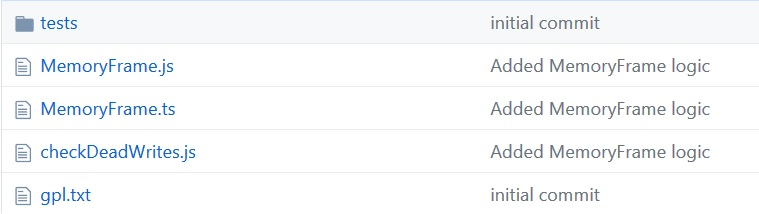
\includegraphics[width=0.8\linewidth]{Github_Content.jpg}
	\caption{Shows which files our project consists of on "Github".}
	\label{img:grafik-dummy}
\end{figure}
\subsection{First Tests to get familar with Jalangi}
\begin{figure}[!htb]
  \centering 
   \subfigure[Level 1...]{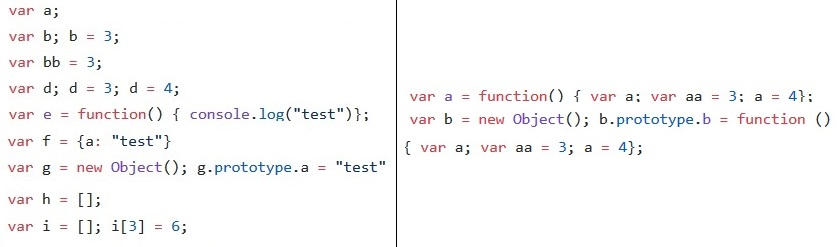
\includegraphics[width=0.4\textwidth]{Level1.jpg}}\qquad 
   \subfigure[Level2...]{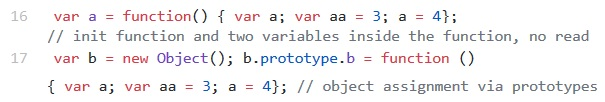
\includegraphics[width=0.4\textwidth]{Level2.jpg}}
  \caption{First Tests to get familar with Jalangi } 
\end{figure}
\subsection{Our Jalangi-Code-Analysis / Algorithm}
\subsection{Sample Applications which contains "Dead-Writes"}
\pagebreak
\section{Results}
\subsection{Problems which occured during our work}
Initially it was a big challenge to familiarize our self with Jalangi. There are exists documentations and introductory examples, but from our personal point of view, they are not really easy to understand.
\subsection{Conclusion}
\subsection{Outlook}
\section{References}
\mbox{-[1]- \url{https://github.com/Samsung/jalangi2}}
\newline
\mbox{-[2]- \url{http://draw.io/}}
\newline
\mbox{-[3]- \url{https://www.teamviewer.com/en/}}
\newline
\mbox{-[4]- \url{https://www.vmware.com}}
\newline
\mbox{-[5]- \url{https://nodejs.org/en/}}




\end{document} 

